\section*{Problem 1}

Three non-self-supporting villages A, B and C in the middle of nowhere consume one food package each per time unit. The required food packages are delivered by a truck, having a capacity of 300 food packages. The locations of the villages are given in the following picture, in which the numbers indicate the distance, more precisely, the number of time units the truck needs to travel from one village to another, including loading or delivering. The truck has to pick up its food packages at location S containing an unbounded supply. The villages only have a limited capacity to store food packages: for A and B this capacity is 120, for C it is 200. Initially, the truck is in S and is fully loaded, and in A, B and C there are 40, 30 and 145 food packages, respectively.

\begin{center}
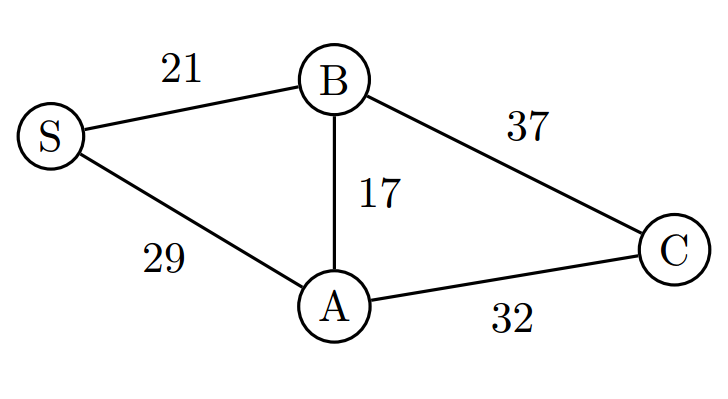
\includegraphics[width=0.45\textwidth]{P1_villages.png}
\end{center}

\begin{description}
  \item[(a)] Show that it is impossible to deliver food packages in such a way that each of the villages consumes one food package per time unit forever.
  \item[(b)]  Show that this is possible if the capacity of the truck is increased to 320 food packages. (Note that a finite graph contains an infinite path starting in a node v if and only if there is a path from v to a node w for which there is a non-empty path from w to itself.)
  \item[(c)]  Figure out whether it is possible if the capacity of the truck is set to 318.
\end{description}

\subsection*{Solution:}

We generalize this problem for $n$ number of villages and a truck with capacity $T$. We introduce $n\times (m+1)$ integer variables $a_{ij}$ for $i=1,...,n$ and $j=0,...,m$, where $m$ is the number of travels that the truck has performed, and $a_{ij}$ represents the number of food packages in the village $i$ after performing $j$ number of travels. We also introduce $m+1$ integer variables $p_j$, $t_j$ and $d_j$ for $j=0,...,m$, where $p_j$ and $t_j$ represent the position of the truck and the number of food packages in it respectively after $j$ number of travels. Finally, $d_j$ depicts the amount of food packages that are delivered to a village just after performing $j$ number of travels.

First we define the boundaries of each variable. To do so, we define $max(i)$ as the maximum number of food packages that village $i$ can store. Then we have the following formula that expresses that the number of food packages in each village should be in the range of zero and its store's capacity:

\[ \bigwedge_{i=1}^n \bigwedge_{j=0}^m 0 \leq a_{ij} \leq max(i).\]

Similarly, we construct the formula for the boundaries of the reminding variables.

\[\bigwedge_{j=0}^m 0 \leq p_j \leq n\;\;\wedge\]
\[\bigwedge_{j=0}^m 0 \leq t_j \leq T\;\;\wedge\]
\[\bigwedge_{j=0}^m 0 \leq d_j.\]

It is worth to mention that $p_j = 0$ means that the truck is in location S (Supplier), whereas $p_j = i$ for $i=1,...,n$ depicts that the truck is in village $i$. Hence, the boundaries of $p_j$ must be in the range of zero and $n$.

The problem specifies the condition that initially the truck is fully loaded and in position S. Additionally, some villages already have an amount of food packages, lets define this initial number of packages as $A_i$ for village $i$. Then we have the following formula:

\[p_0 = 0 \;\;\wedge\]
\[t_0 = T \;\;\wedge\]
\[\bigwedge_{i=0}^n a_{i0} = A_i.\]

Next, we express the condition that the number of delivered packages $d$ in village $i$ is limited by the capacity of this village. Also, when the truck is in position zero (Supplier) it should not deliver any package.

\[\bigwedge_{j=0}^m \bigwedge_{i=1}^n (p_j = i) \rightarrow (d_j \leq (max(i) - a_{ij})) \;\;\wedge\]
\[\bigwedge_{j=0}^m (p_j = 0) \rightarrow (d_j = 0) .\]

Finally, when the truck is in a given position, the next position should be a neighboring village. Also, when moving to another position the amount of food in every village will decrement depending on the travel time. In order to express this conditions, we introduce $\textbf{C}_i$ as the sets of neighbors of village $i$, and the mappings $f_i:\textbf{C}_i \rightarrow \textbf{N}$ to determine the time required to travel from $i$ to one of its neighbor villages, eg. lets say that the set of neighbors of village $1$ is $\textbf{C}_1 = \{0,2\}$ then villages 0 and 2 are connected to village 1, and $f_1(0)$ is the time required to go from village 1 to village 0.

Using all this elements, the formula that expresses this condition is the following:

\[\bigwedge_{j=0}^{m-1} \bigwedge_{i=0}^n (p_j = i) \rightarrow (\bigvee_{k \in \textbf{C}_i} (p_{j+1}=k \;\;\wedge\ a_{ij+1} = a_{ij} + d_{j} - f_i(k) \;\;\wedge\]
\[\qquad \qquad \qquad \bigwedge_{1\leq l \leq n:i\neq l} a_{lj+1} = a_{lj} - f_i(k) \;\;\wedge\]
\[\qquad \qquad(k=0) \rightarrow (t_{j+1} \geq t_j) \;\;\wedge\]
\[\qquad \qquad \qquad \; \;(k\neq0) \rightarrow (t_{j+1} = t_j - d_{j+1}) )).\]

It is worth to mention that the last two expressions of this big formula express that when the selected neighbor is the Supplier ($k=0$), then the next amount of packages in the truck $t$ can only be bigger or equal to the previous one, because in this position the truck is being filled again. When $k \neq 0$ the packages in the truck will decrement since some packages will be delivered to the selected neighbor $k$.

The total formula now consists of the conjunction of all these ingredients. We can find a particular solution for this problem choosing $n = 3$, $T = 300$, $max(1) = max(2) = 120$, $max(3) = 200$, $A_1 = 40$, $A_2 = 30$, $A_3 = 145$, $\textbf{C}_0 = \{1,2\}$, $\textbf{C}_1 = \{0,2,3\}$, $\textbf{C}_2 = \{0,1,3\}$, $\textbf{C}_3 = \{1,2\}$ and the values of $f_i(k)$ as depicted in the picture of the villages.

The complete formula expressed in SMT syntax is as follow:

\vspace{3mm}

\fontfamily{lmtt}\selectfont
{\footnotesize
\noindent
;Practical Assignment - Automated\_ Reasoning 2IMF25\newline
;Problem 1\newline
(benchmark test.smt\newline
:logic QF\_UFLIA\newline
:extrafuns \newline
((a1\_0 Int)  (a2\_0 Int)  (a3\_0 Int)\newline
 (a1\_1 Int)  (a2\_1 Int)  (a3\_1 Int)\newline
 (a1\_2 Int)  (a2\_2 Int)  (a3\_2 Int)\newline
 $\cdots \cdots$
 \newline
 (p\_0 Int)    (t\_0 Int)    (d\_0 Int) \newline
 (p\_1 Int)    (t\_1 Int)    (d\_1 Int)\newline
 (p\_2 Int)    (t\_2 Int)    (d\_2 Int)\newline
 $\cdots \cdots$
\newline
)\newline
:formula \newline
(and\newline
 ;the initial values for each village, the truck and position\newline
 (= p\_0 0)\newline
 (= a1\_0 40) \newline
 (= a2\_0 30) \newline
 (= a3\_0 145)\newline
 (= t\_0 300) \newline
 ;Bound of each variable\newline
 (>= a1\_0 0)  (<= a1\_0 120)  (>= a2\_0 0)  (<= a2\_0 120)  (>= a3\_0 0)  (<= a3\_0 200)\newline
 (>= a1\_1 0)  (<= a1\_1 120)  (>= a2\_1 0)  (<= a2\_1 120)  (>= a3\_1 0)  (<= a3\_1 200)\newline
 (>= a1\_2 0)  (<= a1\_2 120)  (>= a2\_2 0)  (<= a2\_2 120)  (>= a3\_2 0)  (<= a3\_2 200)\newline
 $\cdots \cdots$
\newline
 (>= p\_0 0)  (<= p\_0 3)   (>= t\_0 0)  (<= t\_0 300)   (>= d\_0 0) \newline
 (>= p\_1 0)  (<= p\_1 3)   (>= t\_1 0)  (<= t\_1 300)   (>= d\_1 0) \newline
 (>= p\_2 0)  (<= p\_2 3)   (>= t\_2 0)  (<= t\_2 300)   (>= d\_2 0) \newline
 $\cdots \cdots$
\newline
;Step 1\newline
 (implies (= p\_0 0)  (and (= d\_0 0)\newline
					     (or (and (= p\_1 1) (= a1\_1 (- a1\_0 29)) (= a2\_1 (- a2\_0 29)) (= a3\_1 (- a3\_0 29)) (= t\_1 (- t\_0 d\_1))) \newline
						     (and (= p\_1 2) (= a1\_1 (- a1\_0 21)) (= a2\_1 (- a2\_0 21)) (= a3\_1 (- a3\_0 21)) (= t\_1 (- t\_0 d\_1))))))\newline
							 \newline
 (implies (= p\_0 1)  (and (<= d\_0 (- 120 a1\_0))\newline
					     (or (and (= p\_1 0) (= a1\_1 (- (+ a1\_0 d\_0) 29)) (= a2\_1 (- a2\_0 29)) (= a3\_1 (- a3\_0 29)) (>= t\_1 t\_0)) \newline
						     (and (= p\_1 2) (= a1\_1 (- (+ a1\_0 d\_0) 17)) (= a2\_1 (- a2\_0 17)) (= a3\_1 (- a3\_0 17)) (= t\_1 (- t\_0 d\_1)))\newline
							 (and (= p\_1 3) (= a1\_1 (- (+ a1\_0 d\_0) 32)) (= a2\_1 (- a2\_0 32)) (= a3\_1 (- a3\_0 32)) (= t\_1 (- t\_0 d\_1))))))\newline
\newline
(implies (= p\_0 2)  (and (<= d\_0 (- 120 a2\_0))\newline
					     (or (and (= p\_1 0) (= a1\_1 (- a1\_0 21)) (= a2\_1 (- (+ a2\_0 d\_0) 21)) (= a3\_1 (- a3\_0 21)) (>= t\_1 t\_0)) \newline
						     (and (= p\_1 1) (= a1\_1 (- a1\_0 17)) (= a2\_1 (- (+ a2\_0 d\_0) 17)) (= a3\_1 (- a3\_0 17)) (= t\_1 (- t\_0 d\_1)))\newline
							 (and (= p\_1 3) (= a1\_1 (- a1\_0 37)) (= a2\_1 (- (+ a2\_0 d\_0) 37)) (= a3\_1 (- a3\_0 37)) (= t\_1 (- t\_0 d\_1))))))\newline
							 \newline
(implies (= p\_0 3)  (and (<= d\_0 (- 200 a3\_0))\newline
					     (or (and (= p\_1 1) (= a1\_1 (- a1\_0 32)) (= a2\_1 (- a2\_0 32)) (= a3\_1 (- (+ a3\_0 d\_0) 32)) (= t\_1 (- t\_0 d\_1)))\newline
							 (and (= p\_1 2) (= a1\_1 (- a1\_0 37)) (= a2\_1 (- a2\_0 37)) (= a3\_1 (- (+ a3\_0 d\_0) 37)) (= t\_1 (- t\_0 d\_1))))))\newline
$\cdots \cdots$
\newline
))
}
\fontfamily{helvet}\selectfont

\vspace{3mm}

Now we try to find a solution for each interrogant of the original problem:
\begin{description}
  \item[(a)] Show that it is impossible to deliver food packages in such a way that each of the villages consumes one food package per time unit forever.

  Applying {\tt yices-smt part$2\_1a$.smt}, it yields SAT when choosing $m=20$ but yields UNSAT when generating the code for $m=21$, hence the truck can make at most 20 travels between villages before one consumes all its food. We conclude that is impossible to deliver food packages in such a way that each of the villages consumes one food package per time unit forever.

  \item[(b)]  Show that this is possible if the capacity of the truck is increased to 320 food packages.

  In order to find a solution where the truck can deliver food forever, we first try to find a state that can be reached again in the future, so for this case the truck can perform the same route forever always passing for the same states. We find this adding conditions to the yices' code to compare two different states and yields SAT if they are equal. Performing some experiments we found out that after adding the following formula it yields satisfiable:
  \[a_{1\_10} = a_{1\_3} \;\;\wedge\]
  \[a_{2\_10} = a_{2\_3} \;\;\wedge\]
  \[a_{3\_10} = a_{3\_3} \;\;\wedge\]
  \[a_{1\_10} = a_{1\_3} \;\;\wedge\]

  Choosing $T = 320$ and applying {\tt yices-smt -m part$2\_1b$.smt} to the generated code, the tool yields the following result:

  \fontfamily{lmtt}\selectfont
  {\footnotesize
  \noindent

sat\break
(= t\_0 320)\break
(= a1\_0 40)\break
(= a2\_0 30)\break
(= a3\_0 145)\break
(= d\_0 0)\break
(= p\_0 0)\break
(= t\_1 295)\break
(= a1\_1 19)\break
(= a2\_1 9)\break
(= a3\_1 124)\break
(= d\_1 25)\break
(= p\_1 2)\break
(= t\_2 177)\break
(= a1\_2 2)\break
(= a2\_2 17)\break
(= a3\_2 107)\break
(= d\_2 118)\break
(= p\_2 1)\break
$\cdots \cdots$
  }
  \fontfamily{helvet}\selectfont
  \vspace{3mm}

  Hence we conclude that for the case when the truck has a capacity of 320 food packages, it is possible to deliver food in such a way that each village consumes food forever. The final result for this special case is depicted in the following table:

\newcolumntype{a}{>{\columncolor{yellow}}c}

  \begin{center}
\begin{tabular}{|c|c|c|c|a|c|c|c|c|c|c|a|}
  \hline
  $variables/state$ & 0 & 1 & 2 & 3 & 4 & 5 & 6 & 7 & 8 & 9 & 10  \\
  \hline
  Truck position ($p$) & S & B & A & B & S & A & C & B & S & A & B\\
  Food's pkgs in truck ($t$) & 320 & 295 & 177 & 58 & 320 & 253 & 67 & 0 & 296 & 177 & 58\\
  Food's pkgs delivered ($d$) & 0 & 25 & 118 & 119 & 0 & 67 & 186 & 67 & 0 & 119 & 119\\
  Food's pkgs in village A ($a1$) & 40  & 19  & 2   & 103 & 82 & 53 & 88 & 51  & 30  & 1   & 103 \\
  Food's pkgs in village B ($a2$) & 30  & 9   & 17  & 0   & 98 & 69 & 37 & 0   & 46  & 17  & 0  \\
  Food's pkgs in village C ($a3$) & 145 & 124 & 107 & 90  & 69 & 40 & 8  & 157 & 136 & 107 & 90  \\
  \hline
\end{tabular}
\end{center}

  As can be observed, state 10 is exactly the same as state 3, therefor we have found a route that satisfies the requirement. 

  \item[(c)]  Figure out whether it is possible if the capacity of the truck is set to 318.

  Similarly, we prove that it is possible to deliver food forever for this case too. We generate the yices' code choosing $T = 318$ and adding the same extra condition as in \textbf{b)}, after applying {\tt yices-smt -m part$2\_1c$.smt} it yields the following result:
  
    \fontfamily{lmtt}\selectfont
  {\footnotesize
  \noindent

sat\break
(= t\_0 318)\break
(= a1\_0 40)\break
(= a2\_0 30)\break
(= a3\_0 145)\break
(= d\_0 0)\break
(= p\_0 0)\break
(= t\_1 293)\break
(= a1\_1 19)\break
(= a2\_1 9)\break
(= a3\_1 124)\break
(= d\_1 25)\break
(= p\_1 2)\break
(= t\_2 175)\break
(= a1\_2 2)\break
(= a2\_2 17)\break
(= a3\_2 107)\break
(= d\_2 118)\break
(= p\_2 1)\break
$\cdots \cdots$
  }
  \fontfamily{helvet}\selectfont
  \vspace{3mm}
  
  The following table shows the solution for this problem:
  
\begin{center}
\begin{tabular}{|c|c|c|c|a|c|c|c|c|c|c|a|}
  \hline
  $variables/state$ & 0 & 1 & 2 & 3 & 4 & 5 & 6 & 7 & 8 & 9 & 10  \\
  \hline
  Truck position ($p$) & S & B & A & B & S & A & C & B & S & A & B\\
  Food's pkgs in truck ($t$) & 318 & 293 & 175 & 55 & 318 & 252 & 66 & 0 & 295 & 175 & 55\\
  Food's pkgs delivered ($d$) & 0 & 25 & 118 & 120 & 0 & 66 & 186 & 66 & 0 & 120 & 120\\
  Food's pkgs in village A ($a1$) & 40  & 19  & 2   & 103 & 82 & 53 & 87 & 50  & 29  & 0   & 103 \\
  Food's pkgs in village B ($a2$) & 30  & 9   & 17  & 0   & 99 & 70 & 38 & 1   & 46  & 17  & 0  \\
  Food's pkgs in village C ($a3$) & 145 & 124 & 107 & 90  & 69 & 40 & 8  & 157 & 136 & 107 & 90  \\
  \hline
\end{tabular}
\end{center}
  
\end{description}


\subsection*{Remark:}


\subsection*{Generalization:}




